\documentclass[]{article}
\usepackage{lmodern}
\usepackage{amssymb,amsmath}
\usepackage{ifxetex,ifluatex}
\usepackage{fixltx2e} % provides \textsubscript
\ifnum 0\ifxetex 1\fi\ifluatex 1\fi=0 % if pdftex
  \usepackage[T1]{fontenc}
  \usepackage[utf8]{inputenc}
\else % if luatex or xelatex
  \ifxetex
    \usepackage{mathspec}
  \else
    \usepackage{fontspec}
  \fi
  \defaultfontfeatures{Ligatures=TeX,Scale=MatchLowercase}
\fi
% use upquote if available, for straight quotes in verbatim environments
\IfFileExists{upquote.sty}{\usepackage{upquote}}{}
% use microtype if available
\IfFileExists{microtype.sty}{%
\usepackage{microtype}
\UseMicrotypeSet[protrusion]{basicmath} % disable protrusion for tt fonts
}{}
\usepackage[margin=1in]{geometry}
\usepackage{hyperref}
\hypersetup{unicode=true,
            pdftitle={NOAA Storm Database: Health and Economic Impacts},
            pdfauthor={Kevin Joy},
            pdfborder={0 0 0},
            breaklinks=true}
\urlstyle{same}  % don't use monospace font for urls
\usepackage{color}
\usepackage{fancyvrb}
\newcommand{\VerbBar}{|}
\newcommand{\VERB}{\Verb[commandchars=\\\{\}]}
\DefineVerbatimEnvironment{Highlighting}{Verbatim}{commandchars=\\\{\}}
% Add ',fontsize=\small' for more characters per line
\usepackage{framed}
\definecolor{shadecolor}{RGB}{248,248,248}
\newenvironment{Shaded}{\begin{snugshade}}{\end{snugshade}}
\newcommand{\AlertTok}[1]{\textcolor[rgb]{0.94,0.16,0.16}{#1}}
\newcommand{\AnnotationTok}[1]{\textcolor[rgb]{0.56,0.35,0.01}{\textbf{\textit{#1}}}}
\newcommand{\AttributeTok}[1]{\textcolor[rgb]{0.77,0.63,0.00}{#1}}
\newcommand{\BaseNTok}[1]{\textcolor[rgb]{0.00,0.00,0.81}{#1}}
\newcommand{\BuiltInTok}[1]{#1}
\newcommand{\CharTok}[1]{\textcolor[rgb]{0.31,0.60,0.02}{#1}}
\newcommand{\CommentTok}[1]{\textcolor[rgb]{0.56,0.35,0.01}{\textit{#1}}}
\newcommand{\CommentVarTok}[1]{\textcolor[rgb]{0.56,0.35,0.01}{\textbf{\textit{#1}}}}
\newcommand{\ConstantTok}[1]{\textcolor[rgb]{0.00,0.00,0.00}{#1}}
\newcommand{\ControlFlowTok}[1]{\textcolor[rgb]{0.13,0.29,0.53}{\textbf{#1}}}
\newcommand{\DataTypeTok}[1]{\textcolor[rgb]{0.13,0.29,0.53}{#1}}
\newcommand{\DecValTok}[1]{\textcolor[rgb]{0.00,0.00,0.81}{#1}}
\newcommand{\DocumentationTok}[1]{\textcolor[rgb]{0.56,0.35,0.01}{\textbf{\textit{#1}}}}
\newcommand{\ErrorTok}[1]{\textcolor[rgb]{0.64,0.00,0.00}{\textbf{#1}}}
\newcommand{\ExtensionTok}[1]{#1}
\newcommand{\FloatTok}[1]{\textcolor[rgb]{0.00,0.00,0.81}{#1}}
\newcommand{\FunctionTok}[1]{\textcolor[rgb]{0.00,0.00,0.00}{#1}}
\newcommand{\ImportTok}[1]{#1}
\newcommand{\InformationTok}[1]{\textcolor[rgb]{0.56,0.35,0.01}{\textbf{\textit{#1}}}}
\newcommand{\KeywordTok}[1]{\textcolor[rgb]{0.13,0.29,0.53}{\textbf{#1}}}
\newcommand{\NormalTok}[1]{#1}
\newcommand{\OperatorTok}[1]{\textcolor[rgb]{0.81,0.36,0.00}{\textbf{#1}}}
\newcommand{\OtherTok}[1]{\textcolor[rgb]{0.56,0.35,0.01}{#1}}
\newcommand{\PreprocessorTok}[1]{\textcolor[rgb]{0.56,0.35,0.01}{\textit{#1}}}
\newcommand{\RegionMarkerTok}[1]{#1}
\newcommand{\SpecialCharTok}[1]{\textcolor[rgb]{0.00,0.00,0.00}{#1}}
\newcommand{\SpecialStringTok}[1]{\textcolor[rgb]{0.31,0.60,0.02}{#1}}
\newcommand{\StringTok}[1]{\textcolor[rgb]{0.31,0.60,0.02}{#1}}
\newcommand{\VariableTok}[1]{\textcolor[rgb]{0.00,0.00,0.00}{#1}}
\newcommand{\VerbatimStringTok}[1]{\textcolor[rgb]{0.31,0.60,0.02}{#1}}
\newcommand{\WarningTok}[1]{\textcolor[rgb]{0.56,0.35,0.01}{\textbf{\textit{#1}}}}
\usepackage{graphicx,grffile}
\makeatletter
\def\maxwidth{\ifdim\Gin@nat@width>\linewidth\linewidth\else\Gin@nat@width\fi}
\def\maxheight{\ifdim\Gin@nat@height>\textheight\textheight\else\Gin@nat@height\fi}
\makeatother
% Scale images if necessary, so that they will not overflow the page
% margins by default, and it is still possible to overwrite the defaults
% using explicit options in \includegraphics[width, height, ...]{}
\setkeys{Gin}{width=\maxwidth,height=\maxheight,keepaspectratio}
\IfFileExists{parskip.sty}{%
\usepackage{parskip}
}{% else
\setlength{\parindent}{0pt}
\setlength{\parskip}{6pt plus 2pt minus 1pt}
}
\setlength{\emergencystretch}{3em}  % prevent overfull lines
\providecommand{\tightlist}{%
  \setlength{\itemsep}{0pt}\setlength{\parskip}{0pt}}
\setcounter{secnumdepth}{0}
% Redefines (sub)paragraphs to behave more like sections
\ifx\paragraph\undefined\else
\let\oldparagraph\paragraph
\renewcommand{\paragraph}[1]{\oldparagraph{#1}\mbox{}}
\fi
\ifx\subparagraph\undefined\else
\let\oldsubparagraph\subparagraph
\renewcommand{\subparagraph}[1]{\oldsubparagraph{#1}\mbox{}}
\fi

%%% Use protect on footnotes to avoid problems with footnotes in titles
\let\rmarkdownfootnote\footnote%
\def\footnote{\protect\rmarkdownfootnote}

%%% Change title format to be more compact
\usepackage{titling}

% Create subtitle command for use in maketitle
\providecommand{\subtitle}[1]{
  \posttitle{
    \begin{center}\large#1\end{center}
    }
}

\setlength{\droptitle}{-2em}

  \title{NOAA Storm Database: Health and Economic Impacts}
    \pretitle{\vspace{\droptitle}\centering\huge}
  \posttitle{\par}
    \author{Kevin Joy}
    \preauthor{\centering\large\emph}
  \postauthor{\par}
      \predate{\centering\large\emph}
  \postdate{\par}
    \date{10/15/2019}


\begin{document}
\maketitle

\hypertarget{executive-summary}{%
\subsection{Executive Summary}\label{executive-summary}}

This project involves exploring the U.S. National Oceanic and
Atmospheric Administration's (NOAA) storm database. This database tracks
characteristics of major storms and weather events in the United States,
including when and where they occur, as well as estimates of any
fatalities, injuries, and property damage.

The data analysis addresses the following questions:

\begin{enumerate}
\def\labelenumi{\arabic{enumi}.}
\tightlist
\item
  Across the United States, which types of events (as indicated in the
  \textbf{EVTYPE} variable) are most harmful with respect to population
  health?

  \begin{itemize}
  \tightlist
  \item
    The analysis will demonstrate that the following Events have the
    largest impact on population health

    \begin{enumerate}
    \def\labelenumii{\arabic{enumii}.}
    \tightlist
    \item
      EXCESSIVE HEAT
    \item
      TORNADO
    \item
      FLASH FLOOD
    \item
      RIP CURRENT
    \item
      LIGHTNING
    \item
      HEAT
    \item
      THUNDERSTORM WIND
    \item
      WILDFIRE
    \end{enumerate}
  \end{itemize}
\item
  Across the United States, which types of events have the greatest
  economic consequences?

  \begin{itemize}
  \tightlist
  \item
    The analysis will demonstrate that the following Events have the
    greatest economic consequences

    \begin{enumerate}
    \def\labelenumii{\arabic{enumii}.}
    \tightlist
    \item
      FLOOD
    \item
      HURRICANE/TYPHOON
    \item
      STORM SURGE
    \item
      HAIL
    \item
      FLASH FLOOD
    \item
      TORNADO
    \item
      DROUGHT
    \item
      FROST/FREEZE
    \end{enumerate}
  \end{itemize}
\end{enumerate}

\hypertarget{data-processing}{%
\subsection{Data Processing}\label{data-processing}}

\begin{itemize}
\tightlist
\item
  Load necessary packages
\end{itemize}

\begin{Shaded}
\begin{Highlighting}[]
\KeywordTok{library}\NormalTok{(tidyverse)}
\KeywordTok{library}\NormalTok{(lubridate)}
\end{Highlighting}
\end{Shaded}

\begin{itemize}
\tightlist
\item
  Download data and load csv.bz2 file.
\item
  Since the dataset is large and more recent data is more complete we
  will only load a subset of data to do this analysis.
\end{itemize}

\begin{Shaded}
\begin{Highlighting}[]
\NormalTok{data_url <-}\StringTok{ "https://d396qusza40orc.cloudfront.net/repdata%2Fdata%2FStormData.csv.bz2"}
\NormalTok{dataName <-}\StringTok{ "data/storm.csv.bz2"}
\ControlFlowTok{if}\NormalTok{(}\OperatorTok{!}\KeywordTok{dir.exists}\NormalTok{(}\StringTok{"data"}\NormalTok{))\{}\KeywordTok{dir.create}\NormalTok{(}\StringTok{"data"}\NormalTok{)\}}


\ControlFlowTok{if}\NormalTok{(}\OperatorTok{!}\KeywordTok{file.exists}\NormalTok{(dataName))\{}
    \KeywordTok{download.file}\NormalTok{(data_url, dataName)}
    \CommentTok{#no need to unzip}
\NormalTok{  \}}
\NormalTok{storm_headers <-}\StringTok{ }\KeywordTok{names}\NormalTok{(}\KeywordTok{read.csv}\NormalTok{(dataName, }\DataTypeTok{nrows =} \DecValTok{2}\NormalTok{))}
\NormalTok{storm <-}\StringTok{ }\KeywordTok{read.csv}\NormalTok{(dataName, }\DataTypeTok{header=}\OtherTok{FALSE}\NormalTok{, }\DataTypeTok{skip =}\DecValTok{500000}\NormalTok{)}
\KeywordTok{names}\NormalTok{(storm) <-}\StringTok{ }\NormalTok{storm_headers}
\end{Highlighting}
\end{Shaded}

\begin{itemize}
\tightlist
\item
  Following scripts will clean, filter and normalize the data

  \begin{enumerate}
  \def\labelenumi{\arabic{enumi}.}
  \tightlist
  \item
    Convert dates from factor to dates.
  \end{enumerate}

  \begin{itemize}
  \tightlist
  \item
    Assume the years 2005 - 2010 are representative for the analysis
  \item
    Since 2011 is not a complete year remove 2011
  \end{itemize}
\end{itemize}

\begin{Shaded}
\begin{Highlighting}[]
\NormalTok{storm}\OperatorTok{$}\NormalTok{BGN_DATE <-}\StringTok{ }\KeywordTok{mdy_hms}\NormalTok{(storm}\OperatorTok{$}\NormalTok{BGN_DATE)}
\NormalTok{storm}\OperatorTok{$}\NormalTok{END_DATE <-}\StringTok{ }\KeywordTok{mdy_hms}\NormalTok{(storm}\OperatorTok{$}\NormalTok{END_DATE)}

\CommentTok{#filter to only show values between 2005 and 2010}
\NormalTok{storm <-}\StringTok{ }\KeywordTok{filter}\NormalTok{(storm, BGN_DATE }\OperatorTok{>=}\StringTok{ "2005-01-01"}\NormalTok{, BGN_DATE }\OperatorTok{<}\StringTok{ "2011-01-01"}\NormalTok{)}
\end{Highlighting}
\end{Shaded}

\begin{enumerate}
\def\labelenumi{\arabic{enumi}.}
\setcounter{enumi}{1}
\tightlist
\item
  Normalize Property Damage and Crop Damage to millions by creating new
  variables
\end{enumerate}

\begin{Shaded}
\begin{Highlighting}[]
\NormalTok{exp_key =}\StringTok{ }\KeywordTok{data.frame}\NormalTok{( }\DataTypeTok{key =} \KeywordTok{c}\NormalTok{(}\StringTok{"K"}\NormalTok{, }\StringTok{"M"}\NormalTok{, }\StringTok{"B"}\NormalTok{, }\StringTok{"0"}\NormalTok{, }\StringTok{""}\NormalTok{), }\DataTypeTok{value =} \KeywordTok{c}\NormalTok{(}\DecValTok{1000}\NormalTok{, }\DecValTok{1000000}\NormalTok{, }\DecValTok{1000000000}\NormalTok{, }\DecValTok{10}\NormalTok{, }\DecValTok{0}\NormalTok{))}

\NormalTok{storm}\OperatorTok{$}\NormalTok{PROPDMG_USD_M =}\StringTok{ }\NormalTok{storm }\OperatorTok
\StringTok{  }\KeywordTok{select}\NormalTok{(PROPDMGEXP, PROPDMG) }\OperatorTok
\StringTok{  }\KeywordTok{left_join}\NormalTok{(exp_key , }\DataTypeTok{by =} \KeywordTok{c}\NormalTok{(}\StringTok{"PROPDMGEXP"}\NormalTok{ =}\StringTok{ "key"}\NormalTok{)) }\OperatorTok
\StringTok{  }\KeywordTok{mutate}\NormalTok{(}\DataTypeTok{PROPDMG_USD_M =}\NormalTok{ PROPDMG }\OperatorTok{*}\StringTok{ }\NormalTok{value }\OperatorTok{/}\StringTok{ }\DecValTok{1000000}\NormalTok{) }\OperatorTok
\StringTok{  }\KeywordTok{pull}\NormalTok{()}

\NormalTok{storm}\OperatorTok{$}\NormalTok{CROPDMG_USD_M =}\StringTok{ }\NormalTok{storm }\OperatorTok
\StringTok{  }\KeywordTok{select}\NormalTok{(CROPDMGEXP, CROPDMG) }\OperatorTok
\StringTok{  }\KeywordTok{left_join}\NormalTok{(exp_key , }\DataTypeTok{by=} \KeywordTok{c}\NormalTok{(}\StringTok{"CROPDMGEXP"}\NormalTok{=}\StringTok{"key"}\NormalTok{)) }\OperatorTok
\StringTok{  }\KeywordTok{mutate}\NormalTok{(}\DataTypeTok{CROPDMG_USD_M =}\NormalTok{ CROPDMG }\OperatorTok{*}\StringTok{ }\NormalTok{value }\OperatorTok{/}\StringTok{ }\DecValTok{1000000}\NormalTok{) }\OperatorTok
\StringTok{  }\KeywordTok{pull}\NormalTok{()}
\end{Highlighting}
\end{Shaded}

\begin{verbatim}
## Warning: Column `CROPDMGEXP`/`key` joining factors with different levels,
## coercing to character vector
\end{verbatim}

\hypertarget{results}{%
\subsection{Results}\label{results}}

\begin{itemize}
\tightlist
\item
  Summarize the years of data beween 2005 - 2010 for each Event Type to
  determine total injuries, fatalities, property damage and crop damage
\end{itemize}

\begin{Shaded}
\begin{Highlighting}[]
\NormalTok{storm_impact =}\StringTok{ }\NormalTok{storm }\OperatorTok\StringTok{ }
\StringTok{  }\KeywordTok{group_by}\NormalTok{(EVTYPE) }\OperatorTok\StringTok{ }
\StringTok{  }\KeywordTok{summarize}\NormalTok{(}\DataTypeTok{inj =} \KeywordTok{sum}\NormalTok{(INJURIES),}
            \DataTypeTok{fat =} \KeywordTok{sum}\NormalTok{(FATALITIES),}
            \DataTypeTok{prop=}\KeywordTok{sum}\NormalTok{(PROPDMG_USD_M),}
            \DataTypeTok{crop =} \KeywordTok{sum}\NormalTok{(CROPDMG_USD_M))}
\NormalTok{storm_impact }\OperatorTok\StringTok{ }\KeywordTok{arrange}\NormalTok{(}\KeywordTok{desc}\NormalTok{(fat))}
\end{Highlighting}
\end{Shaded}

\begin{verbatim}
## # A tibble: 57 x 5
##    EVTYPE                    inj   fat       prop     crop
##    <fct>                   <dbl> <dbl>      <dbl>    <dbl>
##  1 EXCESSIVE HEAT           2033   446      3.26   492.   
##  2 TORNADO                  4977   381   5992.     162.   
##  3 FLASH FLOOD               326   312   6087.     684.   
##  4 RIP CURRENT               133   239      0.001    0    
##  5 LIGHTNING                1283   216    372.       1.06 
##  6 HEAT                      611   166      1.52     0.176
##  7 FLOOD                     182   137 123992.    2895.   
##  8 AVALANCHE                  70    96      2.53     0    
##  9 EXTREME COLD/WIND CHILL     7    81      1.13     0    
## 10 THUNDERSTORM WIND        1027    76   3001.     258.   
## # ... with 47 more rows
\end{verbatim}

\hypertarget{types-of-events-that-are-most-harmful-to-population-health}{%
\paragraph{+ Types of events that are most harmful to population
health:}\label{types-of-events-that-are-most-harmful-to-population-health}}

\begin{verbatim}
- Event Types that are in top 90th percentiles for either Injuries or Fatalities between 2005 - 2010

```r
health_impact <- storm_impact %>%
  select(EVTYPE, fat, inj) %>%
  filter(fat > quantile(fat, .9) | inj > quantile(inj, .9)) %>%
  arrange(desc(fat)) %>%
  rename("Fatalities (2005 - 2010)" = fat ,
         "Injuries (2005 - 2010)" = inj )
health_impact
```

```
## # A tibble: 8 x 3
##   EVTYPE            `Fatalities (2005 - 2010)` `Injuries (2005 - 2010)`
##   <fct>                                  <dbl>                    <dbl>
## 1 EXCESSIVE HEAT                           446                     2033
## 2 TORNADO                                  381                     4977
## 3 FLASH FLOOD                              312                      326
## 4 RIP CURRENT                              239                      133
## 5 LIGHTNING                                216                     1283
## 6 HEAT                                     166                      611
## 7 THUNDERSTORM WIND                         76                     1027
## 8 WILDFIRE                                  45                      483
```
\end{verbatim}

\hypertarget{the-following-figure-displays-the-most-devasting-weather-events-for-health-sorted-by-injuries}{%
\subparagraph{The following figure displays the most devasting weather
events for health sorted by
Injuries:}\label{the-following-figure-displays-the-most-devasting-weather-events-for-health-sorted-by-injuries}}

\begin{Shaded}
\begin{Highlighting}[]
\NormalTok{health_impact_long <-}\StringTok{ }\KeywordTok{gather}\NormalTok{(health_impact, }\StringTok{"TYPE"}\NormalTok{, }\StringTok{"VALUE"}\NormalTok{, }\OperatorTok{-}\NormalTok{EVTYPE)}
\KeywordTok{ggplot}\NormalTok{(health_impact_long, }\KeywordTok{aes}\NormalTok{(}\KeywordTok{reorder}\NormalTok{(EVTYPE, VALUE), VALUE, }\DataTypeTok{fill=}\NormalTok{TYPE)) }\OperatorTok{+}
\StringTok{  }\KeywordTok{geom_col}\NormalTok{(}\DataTypeTok{position=}\StringTok{"dodge"}\NormalTok{) }\OperatorTok{+}
\StringTok{  }\KeywordTok{coord_flip}\NormalTok{() }\OperatorTok{+}
\StringTok{  }\KeywordTok{labs}\NormalTok{(}\DataTypeTok{title =} \StringTok{"Health Impact of Major Storms between 2005 - 2010"}\NormalTok{,}
        \DataTypeTok{y =} \StringTok{"# of Injuries / Fatialities"}\NormalTok{,}
        \DataTypeTok{x =} \StringTok{"Event Type"}
\NormalTok{        )}
\end{Highlighting}
\end{Shaded}

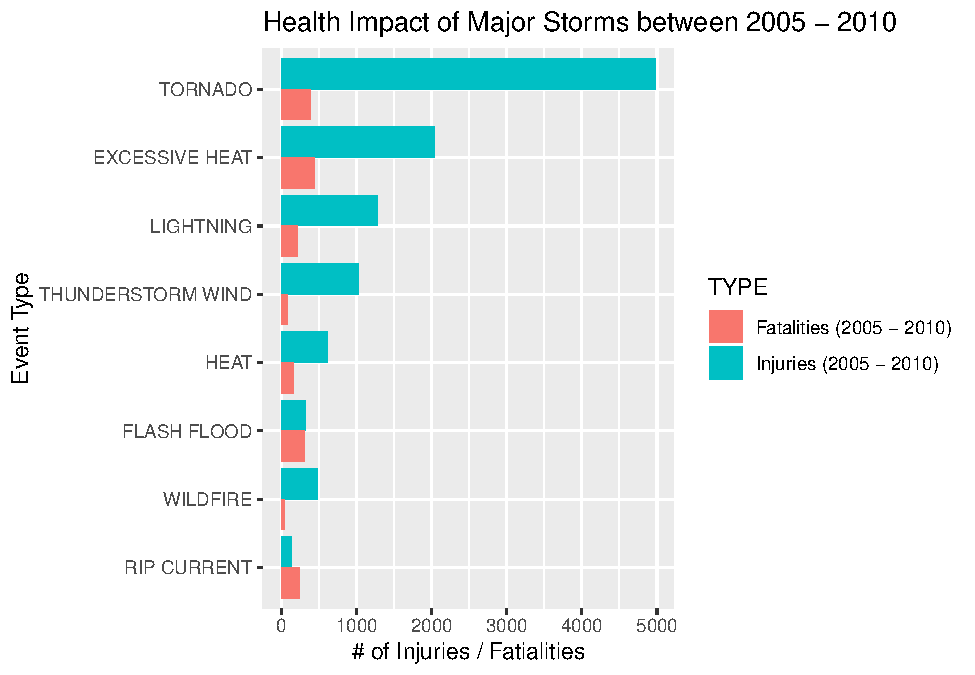
\includegraphics{NOAA_Storm_Analysis_files/figure-latex/unnamed-chunk-7-1.pdf}

\hypertarget{types-of-events-that-have-the-greatest-economic-consequences}{%
\paragraph{+ Types of events that have the greatest economic
consequences:}\label{types-of-events-that-have-the-greatest-economic-consequences}}

\begin{verbatim}
- Event Types that are in top 90th percentiles for either Property or Crop damage between 2005 - 2010

```r
economic_impact <- storm_impact %>%
  select(EVTYPE, prop, crop) %>%
  filter(prop > quantile(prop, .9) | crop > quantile(crop, .9)) %>%
  arrange(desc(prop)) %>%
  rename("Propety Damage $M (2005 - 2010)" = prop ,
         "Crop Damage $M (2005 - 2010)" = crop )
economic_impact
```

```
## # A tibble: 8 x 3
##   EVTYPE          `Propety Damage $M (2005 - 2~ `Crop Damage $M (2005 - 20~
##   <fct>                                   <dbl>                       <dbl>
## 1 FLOOD                               123992.                         2895.
## 2 HURRICANE/TYPH~                      49787.                         2013.
## 3 STORM SURGE                          43059.                            0 
## 4 HAIL                                  7429.                          976.
## 5 FLASH FLOOD                           6087.                          684.
## 6 TORNADO                               5992.                          162.
## 7 DROUGHT                                201.                         4081.
## 8 FROST/FREEZE                             5.44                       1070.
```
\end{verbatim}

\hypertarget{the-following-figure-displays-the-most-economically-impactful-weather-events-sorted-by-property-damage}{%
\subparagraph{The following figure displays the most economically
impactful weather events sorted by property
damage:}\label{the-following-figure-displays-the-most-economically-impactful-weather-events-sorted-by-property-damage}}

\begin{Shaded}
\begin{Highlighting}[]
\NormalTok{economic_impact_long <-}\StringTok{ }\KeywordTok{gather}\NormalTok{(economic_impact, }\StringTok{"TYPE"}\NormalTok{, }\StringTok{"VALUE"}\NormalTok{, }\OperatorTok{-}\NormalTok{EVTYPE)}
\KeywordTok{ggplot}\NormalTok{(economic_impact_long, }\KeywordTok{aes}\NormalTok{(}\KeywordTok{reorder}\NormalTok{(EVTYPE, VALUE), VALUE, }\DataTypeTok{fill=}\NormalTok{TYPE)) }\OperatorTok{+}
\StringTok{  }\KeywordTok{geom_col}\NormalTok{(}\DataTypeTok{position=}\StringTok{"dodge"}\NormalTok{) }\OperatorTok{+}
\StringTok{  }\KeywordTok{coord_flip}\NormalTok{() }\OperatorTok{+}
\StringTok{  }\KeywordTok{labs}\NormalTok{(}\DataTypeTok{title =} \StringTok{"Economic Impact of Major Storms between 2005 - 2010"}\NormalTok{,}
        \DataTypeTok{y =} \StringTok{"$M"}\NormalTok{,}
        \DataTypeTok{x =} \StringTok{"Event Type"}
\NormalTok{        )}
\end{Highlighting}
\end{Shaded}

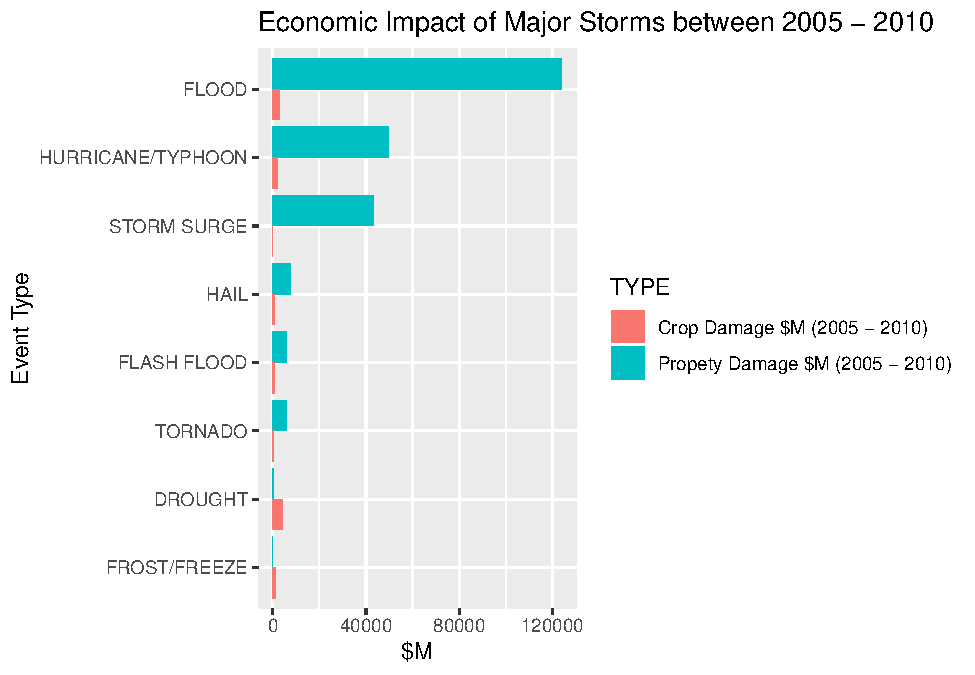
\includegraphics{NOAA_Storm_Analysis_files/figure-latex/unnamed-chunk-9-1.pdf}
*** Better predictions of the aforementioned weather events will lead to
saving lives and the livlihood of people within the United States. ***


\end{document}
